
\section{The Role of Binary Variables}

\begin{frame}
 \frametitle{Categorical Variables}
 \begin{itemize}
   \item Categorical variables provide labels for observations to
denote membership in distinct groups, or categories.
 \item A binary variable is a special case of a categorical variable.
\begin{itemize}
 \item  To
illustrate, a binary variable may tell us whether or not someone has
health insurance.
 \item A categorical variable could tell us whether
someone has (i) private individual health insurance, (ii) private
group insurance, (iii) public insurance or (iv) no health insurance.
\end{itemize}
 \item For categorical variables, there may or may not be an ordering of
the groups.
\begin{itemize}
 \item For health insurance, it is difficult to say which is
``larger,'' private individual versus public health insurance (such
as Medicare).
 \item However, for education, we may group individuals from
a dataset into ``low,'' ``intermediate'' and ``high'' years of
education.
\end{itemize}
 \item Factor is another term used for a (unordered)
categorical explanatory variable.
 \end{itemize}
\end{frame}


\begin{frame}
 \frametitle{Categorical Variables}
 \begin{itemize}
 \item A categorical variable with
$c$ levels can be represented using $c$ binary variables, one for
each category.
\begin{itemize}
 \item For example, from a categorical education variable,
we could code $c$=3 binary variables: (1) a variable to indicate low
education, (2) one to indicate intermediate education and (3) one to
indicate high education.
\end{itemize}
 \item These binary variables are often known as
\emph{dummy variables}.
 \item In regression analysis with an intercept
term, we use only $c$-1 of these binary variables. The remaining
variable enters implicitly through the intercept term.

 \item Through the use of binary variables, we do not make use of the
ordering of categories within a factor.
\begin{itemize}
 \item Because no assumption is
made regarding the ordering of the categories, for the model fit it
does not matter which variable is dropped with regard to the fit of
the model.
 \item However, it does matter for the interpretation of the
regression coefficients.
\end{itemize}
 \end{itemize}
\end{frame}

\begin{frame}
 \frametitle{Example. Term Life Insurance}
 \begin{itemize}
   \item We studied $y$ = LNFACE, the amount that the company will pay in the event
of the death of the named insured (in logarithmic dollars), focusing
on the explanatory variables
 \begin{itemize}
 \item
annual income of the family (LNINCOME, in logarithmic dollars),
 \item the number of years of EDUCATION of the
survey respondent and
 \item the number of household members, NUMHH.
 \end{itemize}
\item We now supplement this by including the categorical variable,
MARSTAT, that is the marital status of the survey respondent. This
may be:
\begin{itemize}
 \item 1, for married
 \item 2, for living with partner
 \item 0, for other (SCF actually breaks this category into
 separated, divorced, widowed, never married and inapplicable, for
 persons age 17 or less or no further persons)
 \end{itemize}

 \end{itemize}
\end{frame}


\begin{frame}[shrink=10]
 \frametitle{Example. Term Life Insurance}
\scalefont{0.9}  \begin{center}  \begin{table}[h] \caption{Summary
Statistics of Logarithmic Face By Marital Status}
\begin{tabular}{lcccc}
\hline
& MARSTAT & Number & Mean & Standard \\
&  &  &  & deviation \\ \hline
Other           & 0 & 47 & 11.01 & 1.455 \\
Married         & 1 & 155 & 12.50 & 1.794 \\
Living together & 2 & 10 & 10.51 & 1.314 \\ \hline
Total           &   & 212 & 12.07 & 1.840 \\
 \hline
\end{tabular}
\end{table}  \end{center}  \scalefont{1.1111}
\begin{figure}[htp]
  \begin{center}
    \includegraphics[width=1\textwidth,angle=270,scale=0.5]{Chapter4/Fig41Boxplot1.ps}
  \end{center}
\end{figure}

\end{frame}

\begin{frame}[shrink=5]
 \frametitle{Example. Term Life Insurance}
  \scalefont{0.9}
  \begin{itemize}
   \item If we run a regression with the binary variables MAR0 and
   MAR2, then
   \begin{eqnarray*}
\widehat{y} &=& 4.915 + 0.308 LNINCOME +0.214 EDUCATION + 0.253
NUMHH \\
 & & ~~ -0.518 MAR0 -1.222 MAR2
\end{eqnarray*}
\begin{itemize}
\item If you are married, then $MAR0=0$, $MAR1=1$ and $MAR2=0$, and
   \begin{eqnarray*}
\widehat{y} &=& 4.915 + 0.308 LNINCOME +0.214 EDUCATION + 0.253
NUMHH
\end{eqnarray*}
\item If living together, then $MAR0=0$, $MAR1=0$ and $MAR2=1$, and
   \begin{eqnarray*}
\widehat{y} &=& 4.915 + 0.308 LNINCOME +0.214 EDUCATION + 0.253
NUMHH -1.222
\end{eqnarray*}
\item The difference in these two equations is $-1.222.$
\end{itemize}
\item Interpret the regression coefficient associated with
$MAR2$ to be the difference in fitted value for someone living
together, compared to a similar person who is married (the omitted
category).
\item Similarly, interpret -0.518 to be the difference between the
``other'' category and the married category.
\item $-0.518 - (-1.222) =0.704$ is the difference between the
other and the living together category.
     \end{itemize}
 \scalefont{1.1111}
\end{frame}




\begin{frame}
 \frametitle{Example. Term Life Insurance}
  \begin{itemize}
   \item Note that $MAR0 + MAR1 + MAR2 = 1$ - there is a $perfect$
   linear dependency among the three.
   \item However, there is not a perfect dependency among any two of
   the three. It turns out that $Cor(MAR0,MAR1) = -0.88$, $Cor(MAR0,MAR2) =
   -0.12$ AND $Cor(MAR1,MAR2) = -0.37$.
   \item Any two out of the three produce the same model in terms of
   goodness of fit
   \end{itemize}
 \begin{table}
 \scalefont{0.9}
\caption{ Term Life ANOVA Table}
\begin{tabular}{lrrr}
 \hline Source
& Sum of Squares & $df$ & Mean Square \\ \hline

Regression & 237.78 & 5 &   47.56 \\
Error      & 476.74 & 206 &  2.31 \\
Total      & 714.52 & 211 &   \\ \hline
\end{tabular}

Residual standard error $s= 1.521$, $R^2 = 33.3\%$, $R_a^2 = 31.7\%$
\scalefont{1.1111}
\end{table}
\end{frame}

\begin{frame}[shrink=10]
 \frametitle{Example. Term Life Insurance}
\begin{table}
\scalefont{0.9} \caption{ Term Life Regression Coefficients}
\begin{tabular}{l|rr|rr|rr}
 \hline
 & \multicolumn{2}{c|}{Model 1}& \multicolumn{2}{c|}{Model 2}& \multicolumn{2}{c}{Model 3}\\
 \hline
 Explanatory & Coefficient & $t$-ratio & Coefficient & $t$-ratio& Coefficient &
 $t$-ratio\\
 Variable &&&&&&\\ \hline
LNINCOME & 0.308 & 3.40 & 0.308 & 3.40 & 0.308 & 3.40 \\
EDUCATION &0.214 & 4.61 &0.214 & 4.61&0.214 & 4.61 \\
NUMHH     & 0.253 & 2.97 & 0.253 & 2.97 & 0.253 & 2.97 \\\hline
Intercept & 3.693& 3.40& 4.915 & 4.58  & 4.397 & 4.50\\
MAR0    &  0.703 &  1.31 &-0.518& -1.71& &\\

MAR1 &  1.222 &   2.41 &  & &0.518 &1.71\\
MAR2 & & & -1.222 & -2.41 & 0.703& -1.31\\
 \hline
\end{tabular}
\scalefont{1.1111}
\end{table}
  \begin{itemize}
   \item Model 2 \emph{appears} the best in the sense that the $t$-ratios are
   larger (in absolute value). The $p$-values are close to
   statistically significant (0.088 for -1.71 and 0.017
   for -2.41).
\item Model 3 \emph{appears} the worst in the sense that the $t$-ratios are
   smaller (in absolute value).
   \item In fact, Model 3 suggests that marital status is not
   statistically significant!!
      \item The three models are equivalent - same estimates, same
      fitted values, as long as you keep your interpretations
      straight.
      \end{itemize}
\end{frame}




\begin{frame}[shrink=5]
 \frametitle{Example. How does Cost-Sharing in Insurance Plans affect
Expenditures in Healthcare?} %\scalefont{0.8}
  \begin{itemize}
   \item Rand Health Insurance Experiment (HIE) - Keeler and Rolph (1988)
\item Cost-Sharing
 \begin{itemize}
\item 14 health insurance plans were grouped by the co-insurance rate (the
percentage paid as out-of-pocket expenditures that varied by 0, 25,
50 and 95\%).
\item One of the 95\% plans limited annual out-of-pocket outpatient
expenditures to \$150 per person (\$450 per family), providing in
effect an individual outpatient deductible. This plan was analyzed
as a separate group.
 \item There were $c=5$ categories of insurance
plans.
 \end{itemize}
 \item Adverse Selection
 \begin{itemize}
\item Individuals choose insurance plans making it difficult to assess
cost-sharing effects.
\item Adverse selection
can arise because individuals in poor chronic health are more likely
to choose plans with less cost sharing, thus giving the appearance
that less coverage leads to greater expenditures.
\item In the Rand HIE,
individuals were randomly assigned to plans, thus removing this
potential source of bias.
 \end{itemize}
     \end{itemize}
  %   \scalefont{1.25}
\end{frame}

\begin{frame}[shrink=10]
 \frametitle{Example. Cost-Sharing in Insurance Plans}
\begin{itemize}
\item Although families were randomly assigned to plans, Keeler and Rolph
(1988) used regression methods to control for participant attributes
and isolate the effects of plan cost-sharing.
\begin{itemize}
\item Based on a sample of $n=1,967$ episode expenditures.
\item Logarithmic expenditure was the dependent variable.
  \end{itemize}
\item Cost-sharing was decomposed into 5
binary variables.
\begin{itemize}
\item These variables are ``Co-ins25,'' ``Co-ins50,''
and ``Co-ins95,'' for coinsurance rates 25, 50 and 95\%,
respectively, and ``Indiv Deductible'' for the plan with individual
deductibles.
\item The omitted variable is the free insurance plan with
0\% coinsurance.
  \end{itemize}
\item The HIE was conducted in six cities; location was decomposed into 5
binary variables: Dayton, Fitchburg, Franklin, Charleston and
Georgetown, with Seattle being the omitted variable.
\item Age and sex was decomposed into 5
binary variables: ``Age 0-2,'' ``Age 3-5,'' ``Age 6-17,'' ``Woman
age 18-65,'' and ``Man age 46-65,'' the omitted category was ``Man
age 18-45.''
\item Other control variables included a health status
scale, socioeconomic status, number of medical visits in the year
prior to the experiment on a logarithmic scale and race.
     \end{itemize}

\end{frame}

\begin{frame}%[shrink=10]
 \frametitle{Example. Cost-Sharing in Insurance Plans}
\begin{table}[h]
\caption{ Coefficients of Episode Expenditures from the Rand HIE}
\scalefont{0.7}
\begin{tabular}{lr|lr}
   \hline
  Variable & Regression &   Variable & Regression \\
           & Coefficient &           & Coefficient \\
\hline
    Intercept &       7.95~ &            &            \\
    Dayton &       0.13* &    Co-ins25 &       0.07~~ \\
 Fitchburg &       0.12~ &    Co-ins50 &       0.02~~ \\
  Franklin &      -0.01~ &    Co-ins95 &      -0.13*~ \\
Charleston &       0.20* &    Indiv Deductible &      -0.03~~ \\
Georgetown &      -0.18* &            &            \\
           &            &            &            \\
Health scale &     -0.02* &    Age 0-2 &      -0.63** \\
Socioeconomic status &  0.03~ &    Age 3-5 &      -0.64** \\
Medical visits &      -0.03~ &   Age 6-17 &      -0.30** \\
Examination &      -0.10* & Woman age 18-65 &       0.11~~ \\
     Black &       0.14* & Man age 46-65 &       0.26~~ \\
 \hline
\multicolumn{4}{l}{Note: * significant at 5\%, ** significant at 1\%} \\
     \multicolumn{4}{l}{\textit{Source}: Keeler and Rolph (1988)} \\
      \hline
\end{tabular}
\scalefont{1.428}
\end{table}

\end{frame}


\begin{frame}[shrink=5]
 \frametitle{Example. Cost-Sharing in Insurance Plans. Findings}
\begin{itemize}
\item
As noted by Keeler and Rolph, there were large differences by site
and age although the regression only served to summarize $R^2=11\%$
of the variability.
\item For the cost-sharing variables, only
``Co-ins95'' was statistically significant, and this only at the 5\%
level, not the 1\% level.
\item
The paper of Keeler and Rolph (1988) examines other types of episode
expenditures, as well as the frequency of expenditures.
\item They
conclude that cost-sharing of health insurance plans has little
effect on the amount of expenditures per episode although there are
important differences in the frequency of episodes.
\begin{itemize}
\item This is because
an episode of treatment is composed of two decisions.
\item The amount of
treatment is made jointly between the patient and the physician and
is largely unaffected by the type of health insurance plan.
\item The
decision to seek health care treatment is made by the patient; this
decision-making process is more susceptible to economic incentives
in cost-sharing aspects of health insurance plans.
  \end{itemize}
  \end{itemize}
\end{frame}




\section{Statistical Inference for Several Coefficients}

\subsection{Sets of Regression Coefficients}

\begin{frame}%[shrink=5]
 \frametitle{Sets of Regression Coefficients}
\begin{itemize}
\item Wish to consider the \emph{joint} effect of regression coefficients.
\begin{itemize}
\item For example, in the Rand HIE, is ``location'' important? This
means examining all of the binary city variables at the same time.
  \end{itemize}
\item Recall the regression coefficients
$\boldsymbol \beta =\left( \beta _{0}, \beta _{1}, \dots,\beta
_{k}\right) ^{\prime },$ a $(k+1)\times 1$ vector.
\item Introduce \textbf{C}, a generic  $p\times (k+1)$ matrix that is
user-specified (and depends on the application)
\item Thus, $\mathbf{C} \boldsymbol
\beta,$ will denote several linear combinations of regression
coefficients
\item Some applications  involve testing whether $\mathbf{C} \boldsymbol \beta$ equals
a specific known value (denoted as \textbf{d}).
\item We call
$H_{0}:\mathbf{C \boldsymbol \beta =d}$ the \emph{general linear
hypothesis}.

  \end{itemize}
\end{frame}

\begin{frame}%[shrink=5]
 \frametitle{Sets of Regression Coefficients. Special Cases}
\begin{itemize}
\item A regression coefficient, say
$\beta_j.$ Choose $p=1$ and \textbf{C} to be a $1\times (k+1$)
vector with a one in the $(j+1)st$ column and zeros otherwise. These
choices result in
\begin{equation*}
\mathbf{C \boldsymbol \beta =}\left( 0~...~0~1~0~...~0\right) \left(
\begin{array}{c}
\beta _{0} \\
\vdots  \\
\beta _{k}%
\end{array}
\right) =\beta_j.
\end{equation*}
\item A linear combination of regression
coefficients. Choose $p=1$ and $\mathbf{C = c^{\prime}}= \left(c_0,
\ldots, c_k \right)^{\prime}$, to get
\begin{equation*}
\mathbf{C} \boldsymbol \beta =\mathbf{c}^{\prime} \boldsymbol \beta
= c_0 \beta_0 + \ldots + c_k \beta_k.
\end{equation*}
For example, if $c_0 = 1, c_1=x_1, \ldots, c_k=x_k$, then
$\mathbf{c}^{\prime} \boldsymbol \beta = c_0 \beta_0 + \ldots + c_k
\beta_k$ = E $y$, the regression function.
  \end{itemize}
\end{frame}

\begin{frame}[shrink=5]
 \frametitle{Sets of Coefficients. Hypothesis Testing}
\begin{itemize}
\item Testing equality of regression
coefficients, say $H_{0}: \beta_1 = \beta_2.$
\begin{itemize}
\item For this purpose, choose
$p=1$, $\mathbf{c}^{\prime}= \left(0,1, -1, 0, \ldots, 0\right),$
and \textbf{d}=0.
\begin{equation*}
\mathbf{C \boldsymbol \beta = c^{\prime} \boldsymbol \beta}=
\left(0,1, -1, 0, \ldots, 0\right) \left(
\begin{array}{c}
\beta _0 \\
\vdots  \\
\beta _k
\end{array}
\right) =\beta_1 - \beta_2 = 0,
\end{equation*}
so that $H_{0}:\mathbf{C \boldsymbol \beta =d}$ becomes $H_{0}:
\beta_1 = \beta_2.$
  \end{itemize}
\item Testing portions of the model. With a \emph{full} regression
function
\begin{equation*}
\mathrm{E~}y=\beta _{0}+\beta _{1}x_{1}...+\beta _{k}x_{k}+\beta
_{k+1}x_{k+1}+...+\beta _{k+p}x_{k+p}
\end{equation*}%
Test the null hypothesis $H_{0}:\beta _{k+1}=...=\beta _{k+p}=0$
\begin{itemize}
\item Choose $\mathbf{d}$ and $\mathbf{C}$ such that
\begin{equation*}
\mathbf{C\boldsymbol \beta =}\left(
\begin{array}{ccccccc}
0 & \cdots  & 0 & 1 & 0 & \cdots  & 0 \\
0 & \cdots  & 0 & 0 & 1 & \cdots  & 0 \\
\vdots  & \vdots  & \vdots  & \vdots  & \vdots  & \ddots  & \vdots  \\
0 & \cdots  & 0 & 0 & 0 & \cdots  & 1%
\end{array}%
\right) \left(
\begin{array}{c}
\beta _{0} \\
\vdots  \\
\beta _{k} \\
\beta _{k+1} \\
\vdots  \\
\beta _{k+p}%
\end{array}%
\right) =\left(
\begin{array}{c}
\beta _{k+1} \\
\vdots  \\
\beta _{k+p}%
\end{array}%
\right) =\left(
\begin{array}{c}
0 \\
\vdots  \\
0
\end{array}%
\right) =\mathbf{d}.
\end{equation*}
  \end{itemize}
  \end{itemize}
\end{frame}


\subsection{The General Linear Hypothesis}

\begin{frame}%[shrink=5]
 \frametitle{The General Linear Hypothesis}
\begin{itemize}
\item Wish to test $H_{0}:\mathbf{C \boldsymbol \beta =d}$.
\item Do this by checking whether $\mathbf{C b -d}$ is close to zero
\begin{itemize}
\item The expected value of $\mathbf{C b -d}$ is $\mathbf{C \boldsymbol \beta -d}.$
\item The variance of  $\mathbf{C b -d}$ is $\sigma^2 \mathbf{C}
\left( \mathbf{X}^{\prime} \mathbf{X} \right)^{-1}
\mathbf{C}^{\prime}.$
\item We use
\begin{equation*}
F-ratio=\frac{(\mathbf{Cb-d)}^{\prime }\left( \mathbf{C}\left(
\mathbf{X^{\prime }X} \right) ^{-1}\mathbf{C}^{\prime }\right)
^{-1}(\mathbf{Cb-d)}}{ps_{full}^{2}}.
\end{equation*}
\begin{itemize}
\item Here, $s_{full}^{2}$ is the mean square error from the full
regression model.
\item Under the null hypothesis, this statistic follows an $F$-distribution with
numerator degrees of freedom $df_{1}=p$ and denominator degrees of
freedom $df_{2}=n-(k+1)$
  \end{itemize}
  \end{itemize}
  \end{itemize}
\end{frame}


\begin{frame}%[shrink=5]
 \frametitle{Procedure for Testing the General Linear Hypothesis}
\begin{itemize}
\item Run the full regression and get the error sum of squares and mean
square error, which we label as $(Error~SS)_{full}$ and
$s_{full}^{2}$, respectively.

\item Consider the model assuming the null hypothesis is true. Run a
regression with this model and get the error sum of squares, which we label $%
(Error~SS)_{reduced}$.

\item Calculate
\begin{equation*}
F-ratio=\frac{(Error~SS)_{reduced}-(Error~SS)_{full}}{ps_{full}^{2}}.
\end{equation*}
\item Reject the null hypothesis in favor of the alternative if the $F$
-ratio exceeds an $F$-value.
\begin{itemize}
\item The $F$-value is a percentile from the
$F$-distribution with $df_{1}=p$ and $df_{2}=n-(k+1)$ degrees of
freedom.
\item Following our notation with the $t$-distribution, we denote
this percentile as $F_{p,n-(k+1),1-\alpha }$, where $\alpha$ is the
significance level.
  \end{itemize} \end{itemize}
\end{frame}



\begin{frame}[shrink=2]
 \frametitle{Example. Term Life Insurance}
   \begin{itemize}
 \item Our first (Chapter 3) regression
   \begin{equation*}
\mathrm{E}y = \beta_0 + \beta_1 LNINCOME +\beta_2 EDUCATION +
\beta_3 NUMHH
\end{equation*}
yielded $s= 1.541$, $R^2 = 30.9\%$, $R_a^2 = 29.9\%$, $Error~SS
=493.84 $.
   \item A regression with the binary variables MAR0 and MAR2,
   \begin{equation*}
\mathrm{E}y = \beta_0 + \beta_1 LNINCOME +\beta_2 EDUCATION +
\beta_3 NUMHH + \beta_4 MAR0 + \beta_4 MAR2
\end{equation*}
yielded $s= 1.521$, $R^2 = 33.3\%$, $R_a^2 = 31.7\%$ , $Error~SS =
476.74$
\item Comparing the two, we have
\begin{eqnarray*}
F-ratio
&=&\frac{(Error~SS)_{reduced}-(Error~SS)_{full}}{ps_{full}^{2}} \\
&=&\frac{493.84 - 476.74 }{2 \times 1.521^2} = 3.696  .
\end{eqnarray*}
\item The degrees of freedom are $df_1 = 2$ and $df_2= 206$.
\item At $\alpha = 5\%$, the $F$-value is $F_{2,206,0.95} =
3.039723$.
\item Thus, we reject $H_0$.
\item The $p$-value is $\Pr( F_{2,206} > 3.696) = 0.0265$.
\end{itemize}
\end{frame}

\begin{frame}[shrink=2]
 \frametitle{Extra Sum of Squares}
   \begin{itemize}
 \item Adding variables to a regression function reduces (never
 increases) the error sum of squares
   \begin{itemize}
\item This is because we are minimizing over additional parameters
\begin{eqnarray*}
(Error~SS)_{full} &=& min_{b_0^{\ast}, \ldots, b_{k+p}^{\ast}}
SS(b_{0}^{\ast },...,b_{k+p}^{\ast }) \\
&=& min_{b_0^{\ast}, \ldots,
b_{k+p}^{\ast}}\sum_{i=1}^{n}\left( y_{i}-\left( b_{0}^{\ast
}+...+b_{k+p}^{\ast }x_{i,k+p}\right) \right)
^{2} \\
&\leq& min_{b_0^{\ast}, \ldots, b_{k}^{\ast}}\sum_{i=1}^{n}\left(
y_{i}-\left( b_{0}^{\ast }+...+b_k^{\ast }x_{i,k}\right) \right)
^{2} \\
&=& (Error~SS)_{reduced}.
\end{eqnarray*}
\item Equivalently, the amount of variability explained increases
(never decreases) because \scalefont{0.9}
\begin{equation*}
(Error~SS)_{reduced}-(Error~SS)_{full}=(Regression~SS)_{full}-(Regression~SS)_{reduced}.
\end{equation*} \scalefont{1.1111}
\item This difference is known as a \emph{Type III Sum of Squares}.
 \end{itemize}
 \end{itemize}
\end{frame}

\begin{frame}[shrink=2]
 \frametitle{F-ratio}
   \begin{itemize}
 \item We can also write
 \begin{eqnarray*}
F-ratio &=&
\frac{(Error~SS)_{reduced}-(Error~SS)_{full}}{ps_{full}^{2}} \\
&=&
\frac{(Regression~SS)_{full}-(Regression~SS)_{reduced}}{ps_{full}^{2}}.
\end{eqnarray*}
\item Dividing the numerator and denominator by $Total~SS$ yields
\begin{equation*}
F-ratio=\frac{\left( R_{full}^{2}-R_{reduced}^{2}\right) /p}{\left(
1-R_{full}^{2}\right) /(n-(k+1))}.
\end{equation*}%
The $F$-ratio measures the statistical significance of the drop in
the coefficient of determination, $R^{2}$.
\item In the special case that $p=1$, one can show that
$(t-ratio)^{2}=F-ratio$. That is, they are equivalent statistics.
  \end{itemize}
\end{frame}


\subsection{Estimating and Predicting Several Coefficients}

\begin{frame}%[shrink=2]
 \frametitle{Estimating Linear Combinations of Regression Coefficients}
   \begin{itemize}
 \item Might wish to estimate $\beta_1 + \beta_2$. (Charitable
 contributions example, represented the expected giving rate per
 unit of income, for income in excess of the Social Security taxable wage base).
 \item More generally, estimate $\mathbf{c}^{\prime} \boldsymbol \beta
= c_0 \beta_0 + \ldots + c_k \beta_k.$
\item Use as a point estimate $\mathbf{c}^{\prime} \mathbf{b}
= c_0 b_0 + \ldots + c_k b_k.$

  \begin{itemize}
 \item This is unbiased and has variance  $\mathrm{Var}\left( \mathbf{c}^{\prime
}\mathbf{b}\right) =\sigma ^{2} \mathbf{c}^{\prime
}(\mathbf{X^{\prime} X})^{-1}\mathbf{c}$.
 \item Thus, the standard error is
 \begin{equation*}
se\left( \mathbf{c}^{\prime }\mathbf{b}\right)
=s\sqrt{\mathbf{c}^{\prime }(\mathbf{X^{\prime }X})^{-1}\mathbf{c}}.
\end{equation*}
\item With this quantity, a $100(1-\alpha ) \%$ confidence interval
for $\mathbf{c}^{\prime } \boldsymbol \beta$ is
\begin{equation*}
\mathbf{c}^{\prime }\mathbf{b}\pm t_{n-(k+1),1-\alpha /2}
~se(\mathbf{c}^{\prime }\mathbf{b}).
\end{equation*}
  \end{itemize}
    \end{itemize}
\end{frame}




\begin{frame}%[shrink=2]
 \frametitle{Prediction Intervals}
   \begin{itemize}
 \item Assume that the set of explanatory variables $
\mathbf{x}^{\ast }$ is known and wish to predict the corresponding response $%
y^{\ast }$.
 \item This new response follows the same assumptions as the observed data.
 \item Specifically, the expected response is $\mathrm{E~}y^{\ast }=%
\mathbf{\mathbf{x}^{\ast }}^{\prime }\boldsymbol \beta $, $\mathbf{\mathbf{x}%
^{\ast }}$ is nonstochastic, $\mathrm{Var~}y^{\ast }=\sigma ^{2}$,
$y^{\ast } $ is independent of $\{y_{1},...,y_{n}\}$ and is normally
distributed.
 \item Under these assumptions, a 100(1-$\alpha $)\%
prediction interval for $y^{\ast }$
\begin{equation*}
\mathbf{\mathbf{x}^{\ast }}^{\prime }\mathbf{b}\pm
t_{n-(k+1),1-\alpha /2} ~s
\sqrt{1+\mathbf{x}^{\ast }{}^{\prime }(\mathbf{X^{\prime }X)}^{-1}\mathbf{x}%
^{\ast }}.
\end{equation*}
This generalizes the prediction interval for introduced in Section
2.4.
    \end{itemize}
\end{frame}

\section{One Factor ANOVA Model}

\subsection{One Factor ANOVA Model}

\begin{frame}%[shrink=2]
 \frametitle{One Factor ANOVA Model}
   \begin{itemize}
    \item Recall that \emph{factor} is another term used for a (unordered)
categorical explanatory variable.
 \item Although factors may be represented as binary variables in a
 linear regression model, we study one factor models as a separate
 unit because
    \begin{itemize}
    \item The method of least squares is much simpler, obviating the
    need to take inverses of high dimensional matrices
    \item The resulting interpretations of coefficients are more
    straightforward
         \end{itemize}
    \item The one factor model is still a special case of the linear
    regression model. Hence, no special statistical theory is needed
    to establish its statistical inference capabilities.
     \end{itemize}
\end{frame}

\begin{frame}[shrink=2]
 \frametitle{Example. Automobile Claims}
   \begin{itemize}
  \item We examine claims experience from a large midwestern (US) property and casualty insurer for private
  passenger automobile experience.
 \item The dependent variable is the amount paid on a closed claim,
 in (US) dollars (claims that were not closed by year end are
 handled separately).
    \item Insurers categorize policyholders according to a risk
    classification system.
  \item The risk classification system is based on
      \begin{itemize}
    \item Automobile operator characteristics (age, gender, marital
    status and whether the primary or occasional driver of a car)
    \item Vehicle characteristics (city versus farm usage, if the vehicle is used to commute to school or
    work, used for business or pleasure, and if commuting, the
    approximate distance of the commute)
     \end{itemize}
\item These factors are summarized by the risk class categorical
variable.
\item Also available is the state in which the claims was filed
(another categorical variable)

     \end{itemize}
\end{frame}

\begin{frame}[shrink=2]
 \frametitle{Example. Automobile Claims}
   \begin{itemize}
    \item Insurers categorize policyholders according to a risk
    classification system.
      \begin{itemize}
    \item The idea behind this is to create groups of policyholders
    with similar risk characteristics that will have similar claims
    experience.
    \item These groups form the basis of the pricing of insurance,
    so that each policyholder is charged an amount that is
    appropriate to their risk category.
  \end{itemize}
\item We will examine only claims that are filed and paid by the
company.
\begin{itemize}
    \item Not based on how frequently
    policyholders have claims.
    \item For rating purposes, the frequency is often more important
    than the severity (amount)
    \item Many insurers decompose their analyses into frequency and
    severity components.
    \item In our analysis, we will not find many explanatory
    variables that are important in explaining claims amounts.
   \end{itemize}
\item However, the one factor ANOVA models can also be used to
analyze claims experience at the policyholder level
\begin{itemize}
    \item Specifically, define $y_i$ to be the amount paid for the
    $i$th policyholder
    \item There will be many zeros here, for policyholders without a
    claim filed during the year.
    \item This is known as the ``pure premium'' approach to rating.
    \end{itemize}
       \end{itemize}
\end{frame}

\begin{frame}[shrink=2]
 \frametitle{Risk Classification Table}

\begin{figure}[htp]
  \begin{center}
    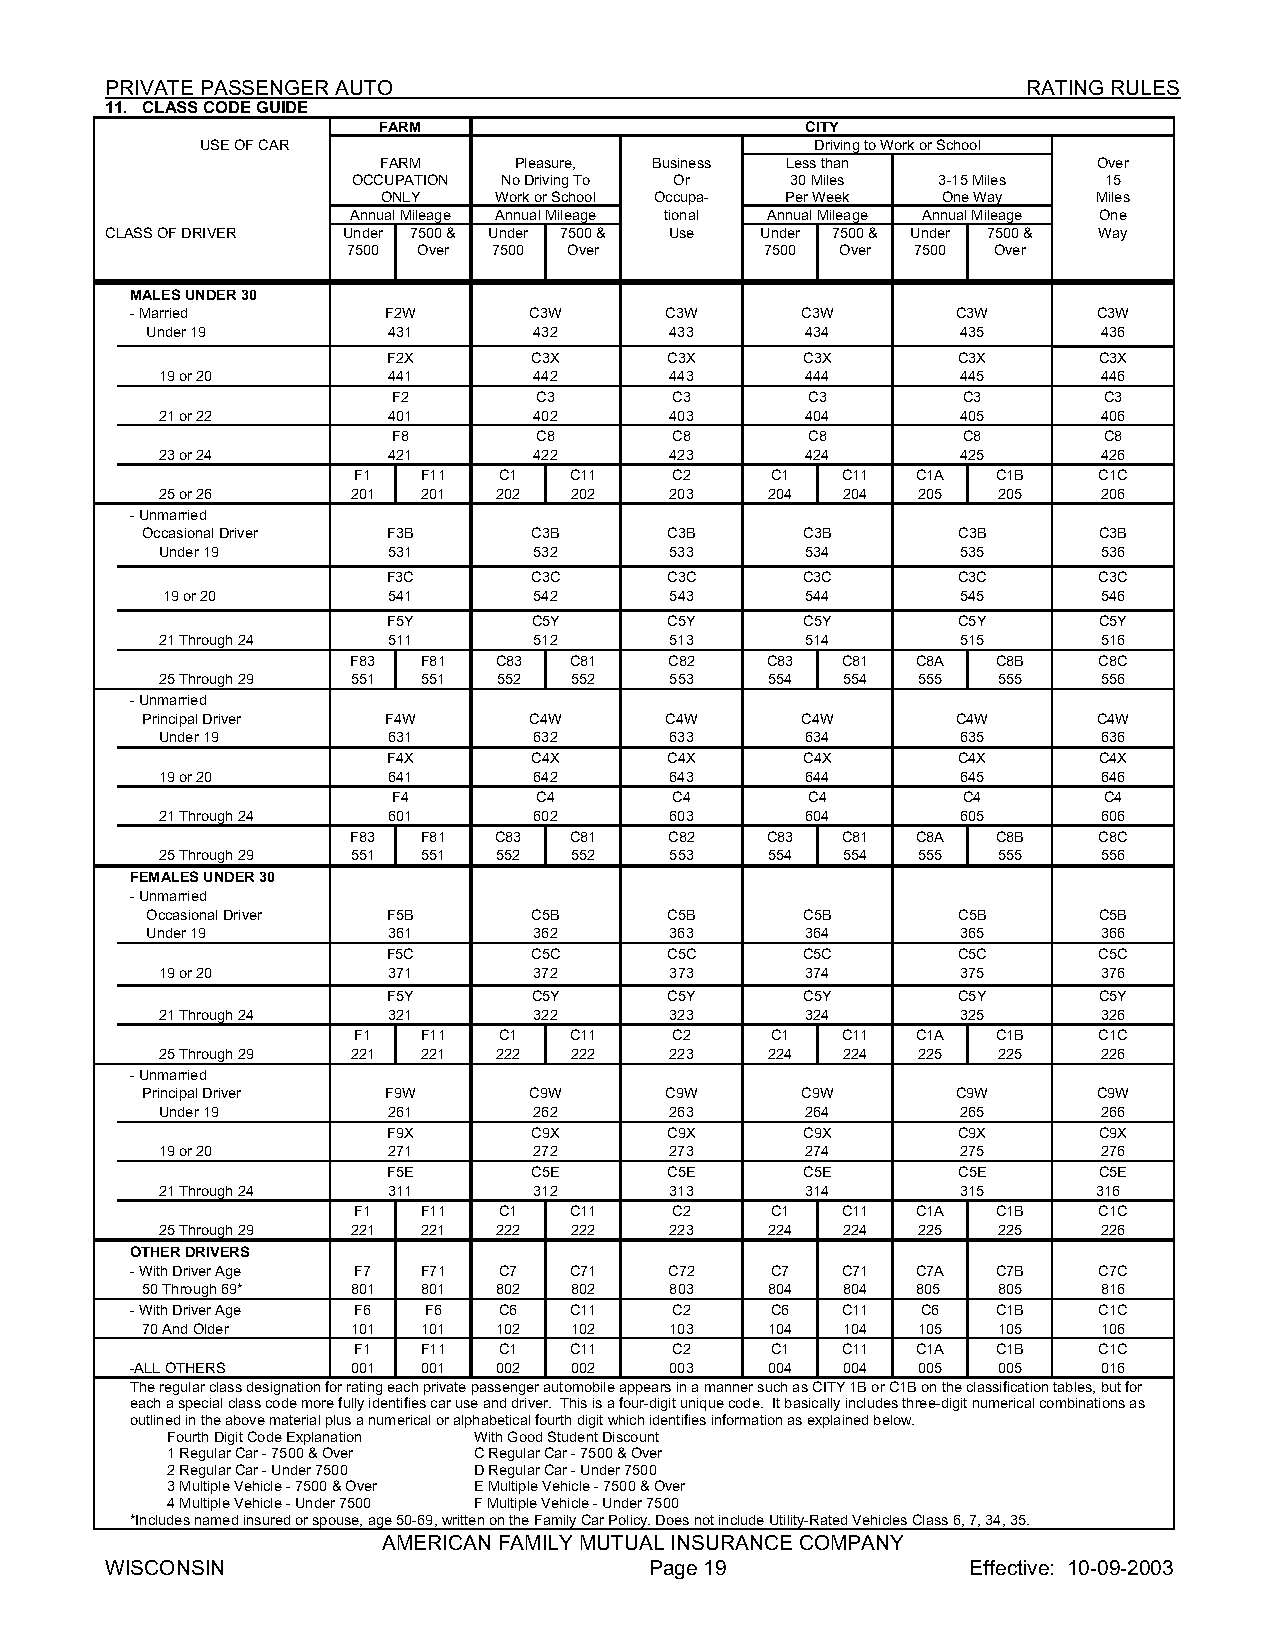
\includegraphics[natheight=5in, natwidth=8in, height=3in,
width=5in]{Chapter4/wiclassonly.pdf}
  \end{center}
\end{figure}
\end{frame}


\begin{frame}%[shrink=2]
 \frametitle{Example. Automobile Claims}
   \begin{itemize}
    \item We consider $n=6,773$ claims from drivers aged 50
    and above
    \item The distribution of claims is very skewed, so we consider
    $y$ = logarithmic claims.
    \item These are from 14 different states
    \item There are 18 risk classes in the table below. This table
    shows little difference in claim amount by risk class.
       \end{itemize}
       \scalefont{0.7}
\begin{tabular}{l|rrrrrrrrr}
\hline
Risk Class &         C1 &        C11 &        C1A &        C1B &        C1C &         C2 &         C6 &         C7 &        C71 \\
 \hline   Number &        726 &       1151 &         77 &        424 &         38 &         61 &        911 &        913 &       1129 \\
   Average &      6.941 &      6.952 &      6.866 &      6.998 &      6.786 &      6.801 &      6.926 &      6.901 &      6.954 \\
 Standard  &      1.064 &      1.074 &      1.072 &      1.068 &      1.110 &      0.948 &      1.115 &      1.058 &      1.038 \\
 ~~Deviation &            &            &            &            &            &            &            &            &            \\
\hline
Risk Class &        C72 &        C7A &        C7B &        C7C &         F1 &        F11 &         F6 &         F7 &        F71 \\
 \hline   Number &         85 &        113 &        686 &         81 &         29 &         40 &        157 &         59 &         93 \\
   Average &      7.183 &      7.064 &      7.072 &      7.244 &      7.004 &      6.804 &      6.910 &      6.577 &      6.935 \\
 Standard  &      0.988 &      1.021 &      1.103 &      0.944 &      0.996 &      1.212 &      1.193 &      0.897 &      0.983 \\
 ~~Deviation &            &            &            &            &            &            &            &            &            \\
\hline
\end{tabular}
  \scalefont{1.4286}

\end{frame}

\begin{frame}[shrink=2]
 \frametitle{Box Plots of Logarithmic Claims by Risk Class}

\begin{figure}[htp]
  \begin{center}
    \includegraphics[width=1\textwidth,angle=270,scale=0.5]{Chapter4/Fig4BoxplotAuto.ps}
  \end{center}
\end{figure}
\end{frame}


\begin{frame}[shrink=2]
 \frametitle{One Factor ANOVA Model}
   \begin{itemize}
    \item Assume that there are $c$ levels of the factor.
    \item At the $j$th level, there are $n_j$ observations. In
    total, there are $n=n_{1}+n_{2}+\ldots +n_{c}$ observations.
    \item The data are:
\begin{center}
\begin{tabular}{cccccc}
Data for Level 1 & \ \ \ \ \ \ \ \ \ \ \ \ \ \ \  & $y_{11}$ &
$y_{21}$ & $
\ldots $ & $y_{n_1,1}$ \\
Data for Level 2 &  & $y_{12}$ & $y_{22}$ & $\ldots $ & $y_{n_2,1}$ \\
. &  & $.$ & $.$ & $...$ & $.$ \\
Data for Level $c$ &  & $y_{1c}$ & $y_{2c}$ & $\ldots $ &
$y_{n_c,c}$
\end{tabular}
\end{center}
\item At the $j$th level, the sample average is
\begin{equation*}
\overline{y}_{j}=\frac{1}{n_{j}}\sum_{i=1}^{n_{j}}y_{ij}.
\end{equation*}
\item The one factor ANOVA model is
\begin{equation*}
y_{ij}=\mu _{j}+ \varepsilon_{ij}\ \ \ \ \ \ i=1,\ldots ,n_{j},\ \ \
\ \ j=1,\ldots ,c.
\end{equation*}
\item With this, use mean $\mu_j$ to be the mean at the $j$th level.
\item Let $\mathrm{Var} y_{ij} = \sigma^2$ be the variance term.
  \end{itemize}
    \end{frame}

\begin{frame}%[shrink=2]
 \frametitle{Method of Least Squares}
   \begin{itemize}
    \item Estimate the parameters $\mu_j,~j=1, \ldots, c$ using least
    squares.
 \begin{itemize}
      \scalefont{0.9}
    \item For candidate estimates $\mu_j^{\ast}$ of $\mu_{j}$, define the sum of squares
\begin{equation*}
SS(\mu_1^{\ast},\ldots
,\mu_c^{\ast})=\sum_{j=1}^{c}\sum_{i=1}^{n_{j}}(y_{ij}-\mu_j^{\ast})^{2}
\end{equation*}
\item Take a derivative with respect to each $\mu_j^{\ast}$, set = 0 and solve. For example,
\begin{eqnarray*}
\frac{\partial}{\partial \mu_1^{\ast}}SS(\hat{\mu}_{1},\ldots
,\hat{\mu}_{c})&=& \frac{\partial}{\partial
\mu_1^{\ast}}\sum_{i=1}^{n_1}(y_{i,1}-\mu_1^{\ast})^{2} =
\sum_{i=1}^{n_1} (-2)(y_{i,1}-\mu_1^{\ast}) = 0.
\end{eqnarray*}
\item Thus, $\bar{y}_1$ is the \textit{least squares estimate }of $\mu
_1$.
\item In general, $\bar{y}_{j}$ is the \textit{least squares estimate }of $\mu
_{j}$.
   \scalefont{1.1111}
  \end{itemize}
  \item This yields least
  squares estimates \emph{without} matrix computations
  \begin{itemize}
     \scalefont{0.9}
    \item Note that here, the dimension of $\mathbf{X^{\prime}X}$ is
    $c \times c$; this is $18 \times 18$ for our auto claims data.
    \item For large auto insurers, common to have
    a risk classification system where $c$ is in the thousands,
    making the usual estimation methods tedious.
     \scalefont{1.1111}
  \end{itemize}
  \end{itemize}

    \end{frame}

\begin{frame}%[shrink=2]
 \frametitle{ANOVA Table for One Factor ANOVA Model}
   \begin{itemize}
    \item Begin with the  \textit{error sum of
squares}
\begin{equation*}
\text{Error SS}=SS(\bar{y}_{1},\ldots ,\bar{y}_{c})=\sum_{j=1}^{c}%
\sum_{i=1}^{n_{j}}(y_{ij}-\bar{y}_{j})^{2}
\end{equation*}%
\item Define the ``Factor'' (Regression) Sum of Squares $\text{Factor SS = Total SS -- Error SS}$
\item To get the
variability decomposition is summarized in the following analysis of
variance (ANOVA) table.

\scalefont{0.9}  \begin{center}  \begin{table}[h] \caption{ ANOVA
Table for One Factor Model}
\begin{tabular}{l|lcc}
\hline Source & Sum of Square & \textit{df} & Mean Square \\
 \hline
Factor & Factor SS &$c-1$ & Factor MS \\
Error &Error SS &$n-c$ & Error MS \\
Total & Total SS & $n-1$ &
 \\ \hline
\end{tabular}
\end{table}  \end{center}  \scalefont{1.1111}
\item The usual (regression) definitions of $R^2$, $s$, and so
forth, hold.
     \end{itemize}

    \end{frame}

    \begin{frame}%[shrink=2]
 \frametitle{Regression and the One Factor ANOVA Model}
   \begin{itemize}
    \item To link the linear (regression) model to the one factor
    ANOVA model:
 \begin{itemize}
    \item For a categorical variable with $c$ levels, define $c$
binary variables, $x_{1},$ $x_{2},\ldots ,x_{c}$.
\item Here,
$x_{j}$ indicates whether or not an observation falls in the $j$th
level. \item Rewrite the one factor ANOVA model $ y=\mu _{j}+
\varepsilon$ as
\begin{equation*}
y=\mu _{1}x_{1}+\mu _{2}x_{2}+\ldots +\mu _{c}x_{c}+\varepsilon.
\end{equation*}

         \end{itemize}
\item To include an intercept term, define $\tau _{j}=\mu _{j}-\mu $,
where $\mu $ is an, as yet, unspecified parameter.
\item The Greek ``t'', $\tau$ is for ``treatment'' effects.
\item With
$x_{1}+x_{2}+\ldots +x_{c}=1$, we have
\begin{equation*}
y=\mu +\tau _{1}x_{1}+\tau _{2}x_{2}+\ldots +\tau
_{c}x_{c}+\varepsilon.
\end{equation*}
\item A simpler expression is
\begin{equation*}
y_{ij}=\mu +\tau_{j} + \varepsilon_{ij}.
\end{equation*}
         \end{itemize}

    \end{frame}


    \begin{frame}%[shrink=2]
 \frametitle{Reparameterizing the One Factor ANOVA Model}
   \begin{itemize}
    \item The one factor ANOVA Model can be expressed as
\begin{equation*}
y_{ij}=\mu +\tau_{j} + \varepsilon_{ij}, ~~~i=1, \ldots, n+j,
~~~j=1,\ldots, c.
\end{equation*}
\item There are $1+c$ parameters, too many (starting with $c$
means). ``Overparameterized.''
\item Two ways to restrict the parameters
   \begin{itemize}
    \item Drop one of the binary variables, for example,
    \begin{equation*}
y=\mu +\tau _{1}x_{1}+\tau _{2}x_{2}+\ldots +\tau
_{c-1}x_{c-1}+\varepsilon.
\end{equation*}
\item Minimize the sum of squares subject to the constraint that the
sum of taus equals zero. More formally, we use the weighted sum
$\sum_{j=1}^{c}n_{j}\tau _{j}=0 $.
      \end{itemize}
         \end{itemize}

    \end{frame}

\subsection{Matrix Expressions}
    \begin{frame}[shrink=2]
 \frametitle{The One Factor ANOVA Model - Matrix Expressions}
   \begin{itemize}
    \item This model can be written as
\begin{equation*}
y=\mu _{1}x_{1}+\mu _{2}x_{2}+\ldots +\mu _{c}x_{c}+\varepsilon.
\end{equation*}
\item Using matrix notation, we have
\begin{equation*}
\mathbf{y}=%
\begin{bmatrix}
y_{1,1} \\
\cdot  \\
\cdot  \\
\cdot  \\
y_{n_{1},1} \\
\cdot  \\
\cdot  \\
\cdot  \\
y_{1,c} \\
\cdot  \\
\cdot  \\
\cdot  \\
y_{n_{c},c}%
\end{bmatrix}%
=%
\begin{bmatrix}
1 & 0 & \cdot \cdot \cdot  & 0 \\
\cdot  & \cdot  & \cdot \cdot \cdot  & \cdot  \\
\cdot  & \cdot  & \cdot \cdot \cdot  & \cdot  \\
\cdot  & \cdot  & \cdot \cdot \cdot  & \cdot  \\
1 & 0 & \cdot \cdot \cdot  & \cdot  \\
\cdot  & \cdot  & \cdot \cdot \cdot  & \cdot  \\
\cdot  & \cdot  & \cdot \cdot \cdot  & \cdot  \\
\cdot  & \cdot  & \cdot \cdot \cdot  & \cdot  \\
0 & 0 & \cdot \cdot \cdot  & 1 \\
\cdot  & \cdot  & \cdot \cdot \cdot  & \cdot  \\
\cdot  & \cdot  & \cdot \cdot \cdot  & \cdot  \\
\cdot  & \cdot  & \cdot \cdot \cdot  & \cdot  \\
0 & 0 & \cdot \cdot \cdot  & 1%
\end{bmatrix}%
\begin{bmatrix}
\mu _{1} \\
\cdot  \\
\cdot  \\
\cdot  \\
\mu _{c}%
\end{bmatrix}%
+%
\begin{bmatrix}
\varepsilon_{1,1} \\
\cdot  \\
\cdot  \\
\cdot  \\
\varepsilon_{n_{1},1} \\
\cdot  \\
\cdot  \\
\cdot  \\
\varepsilon_{1,c} \\
\cdot  \\
\cdot  \\
\cdot  \\
\varepsilon_{n_{c},c}%
\end{bmatrix}%
=\mathbf{X\ \boldsymbol \beta + \boldsymbol \varepsilon} \text{\ \ \
\ }
\end{equation*}
             \end{itemize}
    \end{frame}


    \begin{frame}%[shrink=2]
 \frametitle{The One Factor ANOVA Model - Matrix Expressions}
   \begin{itemize}
    \item We write $\mathbf{0}$ and
$\mathbf{1}$ for a column of zeros and ones, respectively. Thus,

\begin{equation*}
\mathbf{y}=%
\begin{bmatrix}
\mathbf{1}_1 & \mathbf{0}_1 & \cdot \cdot \cdot  & \mathbf{0}%
_{1} \\
\mathbf{0}_{2} & \mathbf{1}_2 & \cdot \cdot \cdot  & \mathbf{0}%
_{2} \\
\cdot  & \cdot  & \cdot \cdot \cdot  & \cdot  \\
\cdot  & \cdot  & \cdot \cdot \cdot  & \cdot  \\
\cdot  & \cdot  & \cdot \cdot \cdot  & \cdot  \\
\mathbf{0}_c & \mathbf{0}_c & \cdot \cdot \cdot  & \mathbf{1}_c
\end{bmatrix}
\begin{bmatrix}
\mu _{1} \\
\mu _{2} \\
\cdot  \\
\cdot  \\
\cdot  \\
\mu _{c}%
\end{bmatrix}%
+\boldsymbol \varepsilon =\mathbf{X \boldsymbol \beta +\boldsymbol
\varepsilon }\text{ \ \ \ }
\end{equation*}
\item Here, $\mathbf{0}_{1}$ and $\mathbf{1}_{1}$ stand for
vector columns of length $n_{1}$ of zeros and ones, respectively.
                 \end{itemize}
    \end{frame}

    \begin{frame}%[shrink=2]
 \frametitle{The One Factor ANOVA Model - Matrix Expressions}
\begin{eqnarray*}
(\mathbf{X^{\prime }X})^{-1} &=&\left(
\begin{bmatrix}
\mathbf{1}_1 & \mathbf{0}_2 & \cdot \cdot \cdot  & \mathbf{0}_c \\
\mathbf{0}_1 & \mathbf{1}_2 & \cdot \cdot \cdot  & \mathbf{0}_c \\
\cdot  & \cdot  & \cdot \cdot \cdot  & \cdot  \\
\cdot  & \cdot  & \cdot \cdot \cdot  & \cdot  \\
\cdot  & \cdot  & \cdot \cdot \cdot  & \cdot  \\
\mathbf{0}_{1} & \mathbf{0}_{2} & \cdot \cdot \cdot  & \mathbf{1}_c%
\end{bmatrix}^{\prime }%
\begin{bmatrix}
\mathbf{1}_1 & \mathbf{0}_1 & \cdot \cdot \cdot  & \mathbf{0}%
_{1} \\
\mathbf{0}_{2} & \mathbf{1}_2 & \cdot \cdot \cdot  & \mathbf{0}%
_{2} \\
\cdot  & \cdot  & \cdot \cdot \cdot  & \cdot  \\
\cdot  & \cdot  & \cdot \cdot \cdot  & \cdot  \\
\cdot  & \cdot  & \cdot \cdot \cdot  & \cdot  \\
\mathbf{0}_{c} & \mathbf{0}_{c} & \cdot \cdot \cdot  & \mathbf{1}_c
\end{bmatrix} \notag
\right) ^{-1} \\
&=&%
\begin{bmatrix}
n_1 & 0 & \cdot \cdot \cdot  & 0 \\
0 & n_2 & \cdot \cdot \cdot  & 0 \\
\cdot  & \cdot  & \cdot \cdot \cdot  & \cdot  \\
\cdot  & \cdot  & \cdot \cdot \cdot  & \cdot  \\
\cdot  & \cdot  & \cdot \cdot \cdot  & \cdot  \\
0 & 0 & \cdot \cdot \cdot  & n_c%
\end{bmatrix}%
^{-1}=%
\begin{bmatrix}
\frac{1}{n_1} & 0 & \cdot \cdot \cdot  & 0 \\
0 & \frac{1}{n_2} & \cdot \cdot \cdot  & 0 \\
\cdot  & \cdot  & \cdot \cdot \cdot  & \cdot  \\
\cdot  & \cdot  & \cdot \cdot \cdot  & \cdot  \\
\cdot  & \cdot  & \cdot \cdot \cdot  & \cdot  \\
0 & 0 & \cdot \cdot \cdot  & \frac{1}{n_c}
\end{bmatrix}%
.
\end{eqnarray*}
    \end{frame}
    \begin{frame}[shrink=10]
 \frametitle{The One Factor ANOVA Model - Matrix Expressions}
   \begin{itemize}
    \item We don't need to calculate least square parameter
    estimates using $\mathbf{(X}^{\prime }\mathbf{X)}^{-1}\mathbf{X}^{\prime
    }\mathbf{y}$, but we can...
\begin{eqnarray*}
\mathbf{b} &=&%
\begin{bmatrix}
\hat{\mu}_{1} \\
\cdot  \\
\cdot  \\
\cdot  \\
\hat{\mu}_{c}%
\end{bmatrix}%
=\mathbf{(X}^{\prime }\mathbf{X)}^{-1}\mathbf{X}^{\prime }\mathbf{y}=%
\begin{bmatrix}
\frac{1}{n_1} & 0 & \cdot \cdot \cdot  & 0 \\
0 & \frac{1}{n_2} & \cdot \cdot \cdot  & 0 \\
\cdot  & \cdot  & \cdot \cdot \cdot  & \cdot  \\
\cdot  & \cdot  & \cdot \cdot \cdot  & \cdot  \\
\cdot  & \cdot  & \cdot \cdot \cdot  & \cdot  \\
0 & 0 & \cdot \cdot \cdot  & \frac{1}{n_c}
\end{bmatrix}
\begin{bmatrix}
\mathbf{1}_1 & \mathbf{0}_2 & \cdot \cdot \cdot  & \mathbf{0}_c \\
\mathbf{0}_1 & \mathbf{1}_2 & \cdot \cdot \cdot  & \mathbf{0}_c \\
\cdot  & \cdot  & \cdot \cdot \cdot  & \cdot  \\
\cdot  & \cdot  & \cdot \cdot \cdot  & \cdot  \\
\cdot  & \cdot  & \cdot \cdot \cdot  & \cdot  \\
\mathbf{0}_{1} & \mathbf{0}_{2} & \cdot \cdot \cdot  & \mathbf{1}_c%
\end{bmatrix} ^{\prime }
\begin{bmatrix}
y_{1,1} \\
\cdot  \\
\cdot  \\
\cdot  \\
y_{n_{1},1} \\
\cdot  \\
\cdot  \\
\cdot  \\
y_{1,c} \\
\cdot  \\
\cdot  \\
\cdot  \\
y_{n_{c},c}%
\end{bmatrix} \notag
\\
&=&%
\begin{bmatrix}
\frac{1}{n_1} & 0 & \cdot \cdot \cdot  & 0 \\
0 & \frac{1}{n_2} & \cdot \cdot \cdot  & 0 \\
\cdot  & \cdot  & \cdot \cdot \cdot  & \cdot  \\
\cdot  & \cdot  & \cdot \cdot \cdot  & \cdot  \\
\cdot  & \cdot  & \cdot \cdot \cdot  & \cdot  \\
0 & 0 & \cdot \cdot \cdot  & \frac{1}{n_c}
\end{bmatrix}
\begin{bmatrix}
\sum_{i=1}^{n_{1}}y_{i1} \\
\cdot  \\
\cdot  \\
\cdot  \\
\sum_{i=1}^{n_{c}}y_{ic}%
\end{bmatrix}%
=%
\begin{bmatrix}
\bar{y}_{1} \\
\cdot  \\
\cdot  \\
\cdot  \\
\bar{y}_{c}%
\end{bmatrix}%
\end{eqnarray*}
                     \end{itemize}
    \end{frame}


\section{Combining Categorical and Continuous Explanatory Variables}


\begin{frame}%[shrink=10]
\frametitle{Combining a Factor and Covariate}
\begin{itemize}
\item When combining, we use the
terminology \emph{factor} for the categorical variable and
\emph{covariate} for the continuous variable.
\item Here are several different approaches for combining these
variables

\begin{table}[h] \caption{Combinations of One Factor and One Covariate}
\scalefont{0.8}
\begin{tabular}{ll}
\hline Model Description & Notation \\ \hline One factor ANOVA (no
covariate model) &
$y_{ij}=\mu _{j}+\varepsilon_{ij}$ \\
Regression with constant intercept and slope  & $y_{ij}=\beta _{0}+\beta _{1}x_{ij}+\varepsilon_{ij}$ \\
~~(no factor model) \\
Regression with variable intercept and constant slope &
$y_{ij}=\beta _{0j}+\beta _{1}x_{ij}+\varepsilon_{ij}$ \\
~~~(analysis of covariance model) &  \\
Regression with constant intercept and variable slope &
$y_{ij}=\beta _{0}+\beta _{1j}x_{ij}+\varepsilon_{ij}$ \\
Regression with variable intercept and slope &
$y_{ij}=\beta _{0j}+\beta _{1j}x_{ij}+\varepsilon_{ij}$ \\
\hline
\end{tabular}
 \scalefont{1.25}
\end{table}
\end{itemize}
\end{frame}



\begin{frame}%[shrink=10]
\frametitle{Combining a Factor and Covariate}
\begin{figure}[htp]
  \begin{center}
    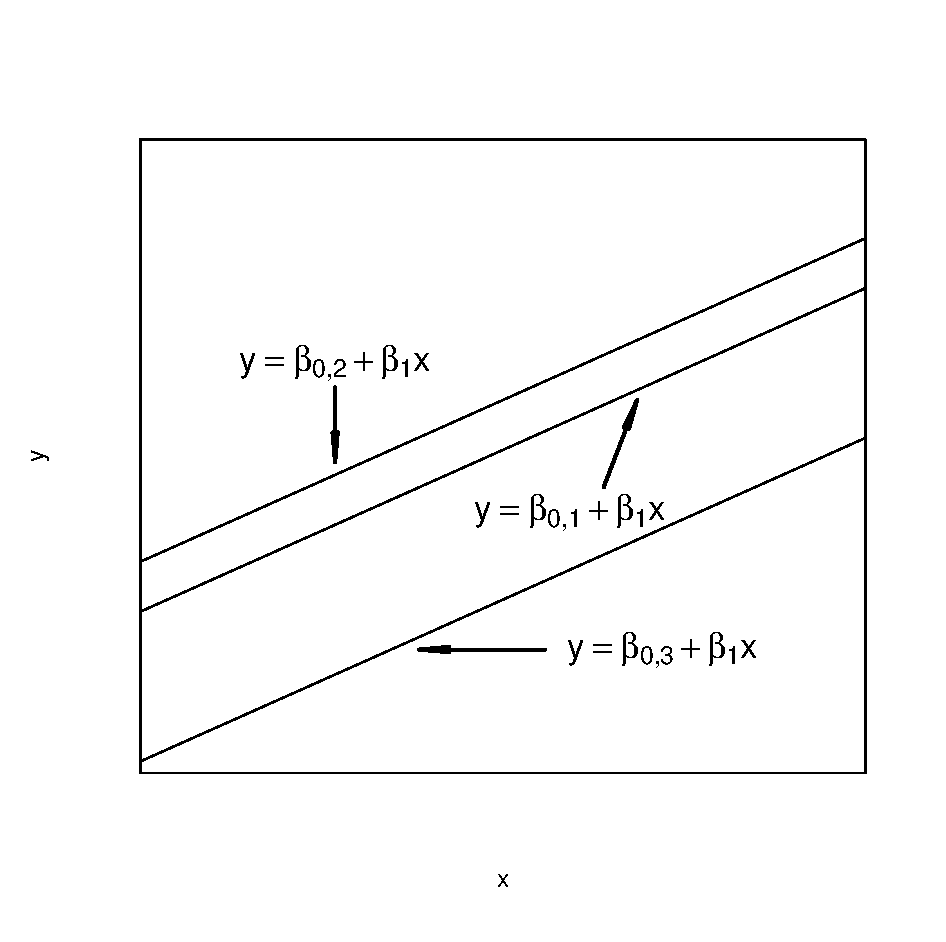
\includegraphics[width=1\textwidth,angle=0,scale=0.45]{Chapter4/Fig4_5A.ps}
    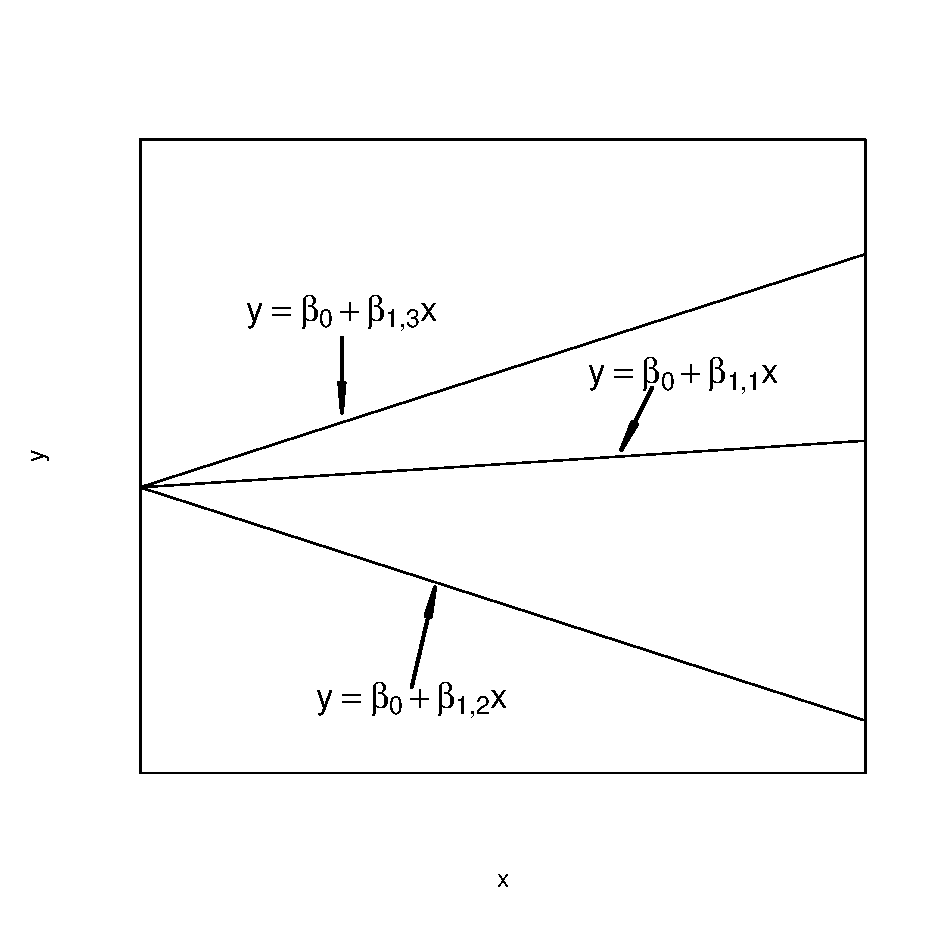
\includegraphics[width=1\textwidth,angle=0,scale=0.45]{Chapter4/Fig4_6A.ps} \hfill
     \parbox[t]{2in}{\caption{ \tiny  Plot of the expected response versus the covariate for the regression model
with variable intercept and constant slope.}} \hfill
    \parbox[t]{2in}{\caption{ \tiny  Plot of the expected response versus the covariate for the regression model
with constant intercept and variable slope.}}
  \end{center}
\end{figure}
\end{frame}

\begin{frame}%[shrink=10]
\frametitle{Combining a Factor and Covariate}
\begin{figure}[htp]
  \begin{center}
    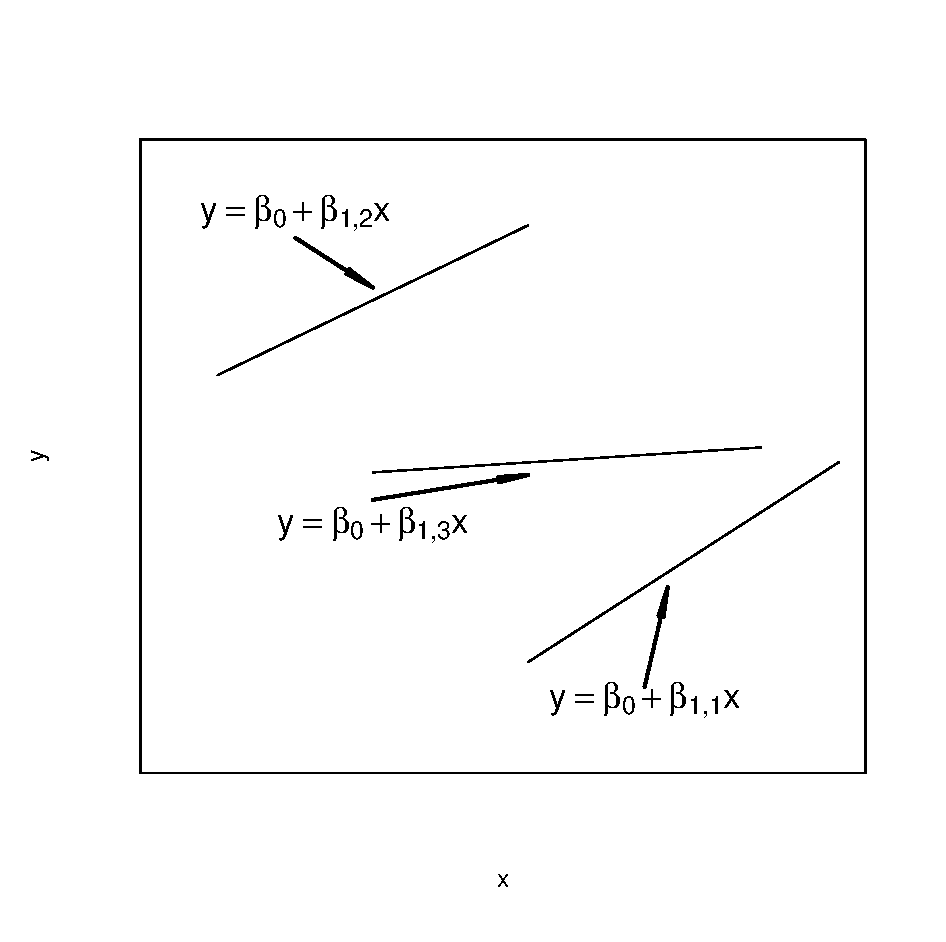
\includegraphics[width=1\textwidth,angle=0,scale=0.5]{Chapter4/Fig4_7A.ps}
    \caption{\label{F4:TheoryVarIntVarSlope} \small  Plot of the expected response versus the covariate for the regression model
with variable intercept and variable slope.}
  \end{center}
\end{figure}
\end{frame}


\begin{frame}[shrink=10]
\frametitle{General Linear Model}
\begin{itemize}
\item In the general linear model
$ y=\beta _{0}+\beta _{1}x_{1}+\ldots \ +\beta _{k}x_{k} +
\varepsilon,$
\begin{itemize}
\item each explanatory variable may be continuous or
categorical
\item The categorical variables are decomposed into binary variables
(typically dropping one for identifiability)
\item Interactions between continuous and categorical variables are
interpreted to be slopes that vary by the level of the category.
\item Interactions between categorical variables are interpreted to
be as creating a new categorical variable
\end{itemize}
\item Example, take gender [male versus female] and
categorical age [young, middle, old], for six combinations of gender
and age.
\begin{itemize}
\item The binary variables $x_1=$(gender=female), $x_2=$(age=young) and
$x_3=$(age=middle) are known as ``main effects.''
\item We can incorporate two interaction variables
$x_4=$(gender=female)*(age=young) and
$x_5=$(gender=female)*(age=middle)
\item This gives five binary variables needed to represent age and gender.

\scalefont{0.9}  \begin{center}
\begin{tabular}{lc|ccccc|c}
\hline Gender & Age & $x_1$ & $x_2$ &  $x_3$ &  $x_4$ &  $x_5$ & $
\mathrm{E~}y=\beta_0 + \beta_1 x_1+ \beta_2 x_2+ \beta_3 x_3+
\beta_4 x_4+ \beta_5 x_5$
\\
\hline
Male & Young    & 0 & 1 & 0 & 0 & 0 & $\beta_0 +\beta_2$\\
Male & Middle   & 0 & 0 & 1 & 0 & 0 & $\beta_0 +\beta_3$\\
Male & Old      & 0 & 0 & 0 & 0 & 0 & $\beta_0 $\\
Female & Young  & 1 & 1 & 0 & 1 & 0 & $\beta_0 +\beta_1+\beta_2+\beta_4$\\
Female & Middle & 1 & 0 & 1 & 0 & 1 & $\beta_0 +\beta_1+\beta_3+\beta_5$\\
Female & Old    & 1 & 0 & 0 & 0 & 0 & $\beta_0 +\beta_1$\\
 \hline
\end{tabular}
 \end{center}  \scalefont{1.1111}




\end{itemize}
\end{itemize}
\end{frame}
